
\chapter{Current System and Proposals, Requirements and Design of New System}\label{sec:currentsystemandproposals}
In this chapter, Section~\ref{sec:currentsystem} is aimed to discuss the design/architecture and user interface of the current system and 
Section~\ref{section:goodexpert} is aimed to introduce expert search indicators of the new system and its design/architecture.

\section{Current System}\label{sec:currentsystem}
This section is intended to give some statistics and briefly discuss design of the current system. Table~\ref{table:currentstats} gives statistics 
of current system.
\begin{table}
\centering
\scalebox{0.5}{\begin{tabular}{|c|c|}
\hline Number of experts & 1569 \\
\hline Number of publications & 22225 \\
\hline Number of all documents   & 24823 \\ 
\hline Number of tokens (terms) & 6876832 \\
\hline
\end{tabular}
}
\caption{Statistics of Current System} \label{table:currentstats}
\end{table}

\begin{figure}
 \centering
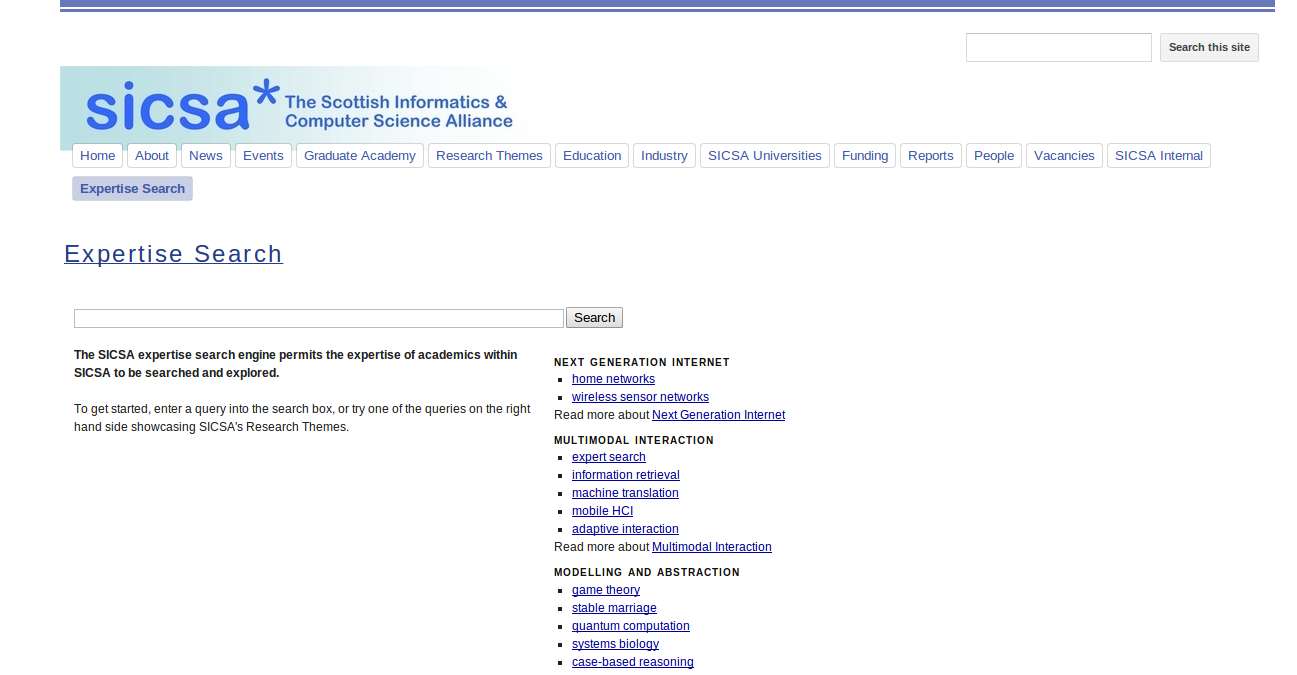
\includegraphics[width=13cm,height=10cm,keepaspectratio]{./figures/oldsicsa.png}
 \caption{Home Page} \label{fig:oldsicsa} 
 \end{figure}
 \begin{figure}
 \centering
 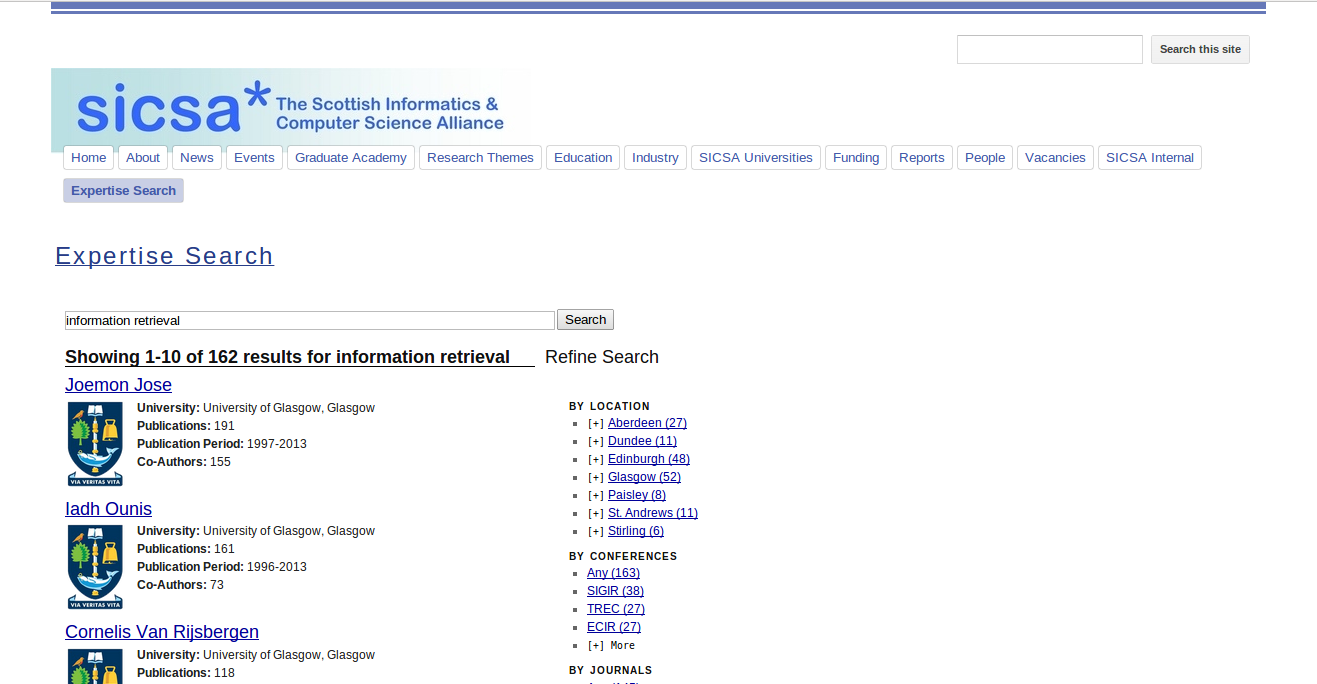
\includegraphics[width=13cm,height=10cm,keepaspectratio]{./figures/oldsearch.png}
 \caption{Experts In Response to ``information retrieval'' Query} \label{fig:resultspage} 
 \end{figure}
 \begin{figure}
 \centering
 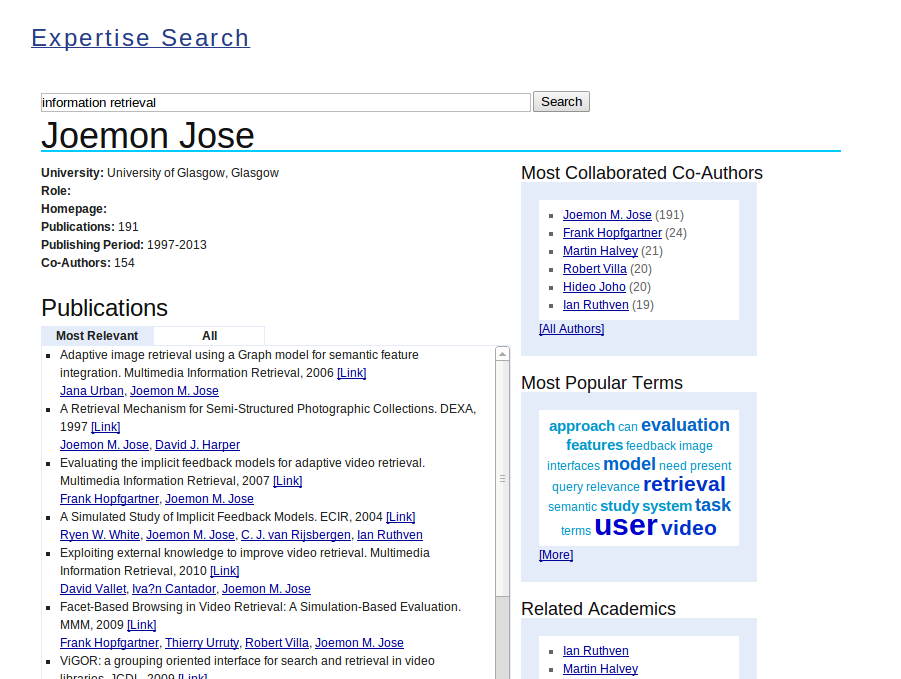
\includegraphics[width=13cm,height=10cm,keepaspectratio]{./figures/oldProfilePage.png}
 \caption{Current Expert's Profile Facet} \label{fig:profilepage} 
\end{figure}
Figure~\ref{fig:oldsicsa} is the home page of SICSA. It provides a set of sample queries categorised in 4 different categories on the right of the 
search panel. The top panel shows links to different SICSA pages. The middle panel is the search panel. It is independent of other panels. 
Experts (results) with respect to a query are independently shown in this panel without reloading other panels. Figure~\ref{fig:resultspage} shows
the interface when experts with respect to a query, ``information retrieval'' are shown. Also, the system demonstrates 
faceted search for academics by presenting refinement options using university, location and total publication range categories.
Below the refinement options is popular tags (terms) appearing in expert's profiles.
Each result in the search panel includes expert's details: university, number of publications, publication period and total number of coauthors.

Figure~\ref{fig:profilepage} illustrates a profile page of an expert. This page introduces most collaborated coauthors facet on the right of the page, a 
facet that shows popular terms appearing in an expert's profile and publications and related academics facet.

\paragraph{Design and Architecture of Current System} \hspace{0pt} \\

 \begin{figure}
 \centering
 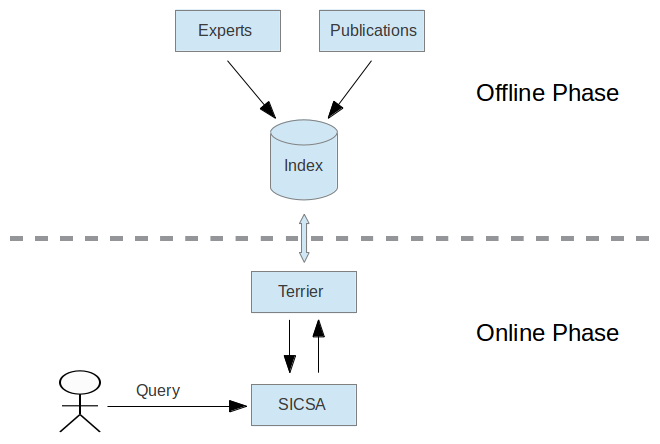
\includegraphics[scale=0.5,keepaspectratio]{./figures/currentSystemDesign.jpg}
 \caption{Design of Current System} \label{fig:currentDesign} 
\end{figure}
Figure~\ref{fig:currentDesign} shows design and architecture of the current system. It makes use of publication as expertise evidence. 
From the figure, after a user submits a query to the system, the system sends a query to Terrier. Terrier then processes the query using publication
as expertise evidence. During this process, $PL2$ retrieval model and voting technique $expCombMNZ$ are applied to calcuate the score of each expert.
The score of each expert is computed using equation~\ref{eq:expCombMNZ} where $score_d$ is the score of expert using $PL2$ retrieval model.
Finally Terrier returns relevant experts to the user.

\section{Expert Search Indicators of the New System}\label{section:goodexpert}
As discussed in Chapter~\ref{section:aims}, this project makes use of publications and funded projects as 
expertise evidence. Based on these evidence, what makes an expert a good expert? we propose several intuitions about a relevant expert as follows 
\begin{itemize}
 \item he has published a lot of publications.
 \item he has co-authored with a lot of other experts in publications.
 \item he has co-authored with a lot of other experts in funded projects.
 \item he has received a lot of funding.
 \item he has involved in a lot of projects.
\end{itemize}

Reasons why such intuitions are chosen are because experts are likely to be professional if they have all intuitions described above. To give an example,
If an expert is looking for co-workers for a project related to information retrieval, he of course would look for co-workers who have experience 
(published lots of publications, involved in lots of projects, etc) and received lots of funding in the field of interest.
It can be seen clearly that these intuitions or features in learning to rank are independent of the query a user submits. These features are query independent
(see Chapter~\ref{section:queryindependent}). However, query dependent features (see Chapter~\ref{section:querydependent}) are taken into account as well. 
In this project, there are 2 query dependent features: 
\begin{itemize}
 \item An expert has published publications on the topic of query (Current System)
 \item An expert has been involved in projects on the topic of query
\end{itemize}

To sum up, a good expert should have high scores in both query dependent and independent features.

\subsection{Requirements Specification}\label{sec:requirements}
Due to the scope of the project it would be impossible to start without a clear vision of how
the end product should function. These requirements were decided on during the early stages of the project. 
The reasoning behind them comes primarily from a number of sources:
\begin{itemize}
 \item Research into a previous attempt at current SICSA system (Section~\ref{sec:currentsystem}).
 \item Research into presenting query results (Section~\ref{sec:presentingQueryResult}).
 \item Research into learning to rank techniques to enhancing the performance of the retrieval system by integrating different kinds of 
 expertise evidence (Section~\ref{sec:letor}).
 \item Discussion with Dr. Craig Macdonald.
\end{itemize}
% However, developing an IR system is researched based. Utilizing learning to rank technique might not 
% produce optimal ranking due to the lack of training dataset. Therefore, 
The requirements have been split into 2 sections depending on their necessity: functional requirements and non-functional requirements

\subsubsection{Functional Requirements}
\paragraph{Must Have} \hspace{0pt} \\
\begin{itemize}
 \item Extracting funded projects from 2 different sources: Grant on the Web~\cite{gow} and Research Councils UK~\cite{gtr}.
 \item Integrating publications and funded projects as expertise evidence.
 \item Utilizing learning to rank techniques with an attempt to improve the effectiveness of the retrieval system using AdaRank and Coordinate Ascent algorithms.
\end{itemize}

\paragraph{Should Have} \hspace{0pt} \\
\begin{itemize}
 \item Refinement options for users to filter results by funded projects, publications and both.
 \item Refinement options for users to filter funded projects and publications of each expert.
\end{itemize}

\paragraph{Could Have} \hspace{0pt} \\
\begin{itemize}
 \item Applications of more LETOR algorithms such as LambdaMART, Random Forests etc.
\end{itemize}

\paragraph{Would Like to Have} \hspace{0pt} \\
\begin{itemize}
 \item Ability to upload funded projects manually by members of the system.
\end{itemize}

\subsubsection{Non-functional Requirements}
\begin{itemize}
 \item Functional 24 hours a day.
 \item Update data regularly.
 \item Able to load all evidence into main memory for efficient lookup.
 \item Fully functional for the purpose of the final demonstration.
\end{itemize}

\subsection{Design and Architecture of New System} \label{section:union}
Figure~\ref{fig:newDesign} shows design of the new system. It makes use of learning to rank (LETOR) technique to integrate 
both publications and funded projects as expertise evidence. From the figure, in contrast to the current system, 
LETOR is applied to documents retrieved from Terrier. This LETOR reranks the documents to get the optimal ranking.

 \begin{figure}
 \centering
 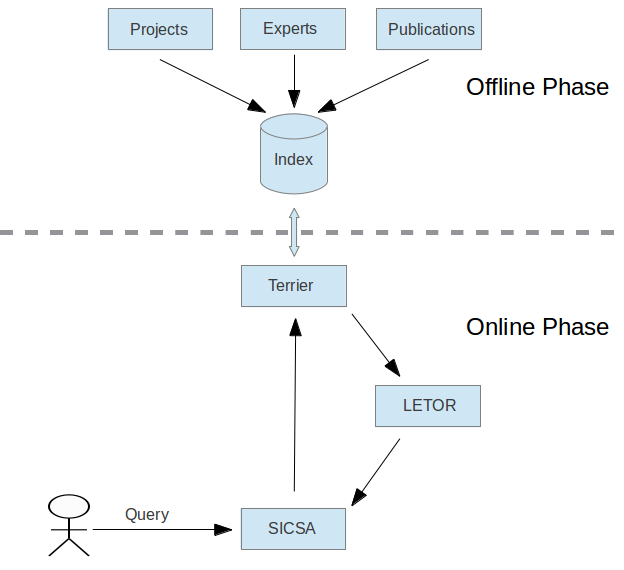
\includegraphics[scale=0.4,keepaspectratio]{./figures/newSystemDesign.png}
 \caption{Design of Current System} \label{fig:newDesign} 
\end{figure}

\paragraph{Retrieving Documents (Experts) with Respect to a Query} \hspace{0pt} \\

\begin{figure}
\centering
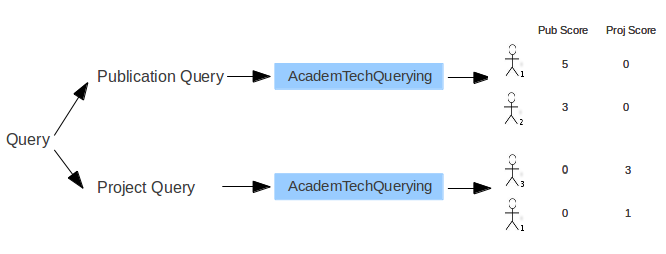
\includegraphics[scale=0.4]{./figures/querying.png}
\caption{Querying} \label{fig:quering} 
\end{figure}
\quad
\begin{figure}
\centering
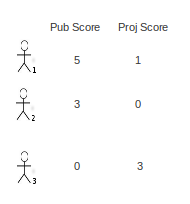
\includegraphics[scale=0.7]{./figures/union.png}
\caption{Results After Union} \label{fig:union} 
\end{figure}
In the previous section, we gave a broad view of the new system retrieval scheme. In this section, we will be more specific on how we are going to 
obtain results from user query before applying them to learning to rank technique to obtain optimal ranking.
Figure~\ref{fig:quering} shows the process of obtaining documents (experts) with respect to a query. 

Given a query $\vec{q}$, it is transformed into publication query $\vec{q}_{pub}$, using only publications as expertise evidence and project
query $\vec{q}_{proj}$, using only funded projects as expertise evidence. 
AcademTechQuerying Class then processes both $\vec{q}_{pub}$ and $\vec{q}_{proj}$. For each query, the system applies $PL2$
retrieval model and voting technique $expCombMNZ$ (see Section~\ref{sec:currentsystem}). The results of both
queries are then unioned, denoted $R_{cand}(\vec{q})$ as shown in Figure ~\ref{fig:union}. The results obtained are based on query dependent features 
as discussed in Chapter~\ref{section:querydependent}. This process is depicted mathematically as follows:

\begin{equation}
 \vec{q}_{pub} \rightarrow R_{cand}(\vec{q}_{pub}),  \vec{q}_{proj} \rightarrow R_{cand}(\vec{q}_{proj})
\end{equation}

\begin{equation}
 R_{cand}(\vec{q}) = R_{cand}(\vec{q}_{pub})\cup R_{cand}(\vec{q}_{proj})
\end{equation}

where $R_{pub}(\vec{q}_{pub})$ and $R_{proj}(\vec{q}_{proj})$ are the rankings of candidate with respect to $\vec{q}_{pub}$ and $\vec{q}_{proj}$
respectively.

\paragraph{Applying a Learned Model and Producing Final Ranking} \hspace{0pt} \\
In the previous section, we discussed how ranking of candidates is obtained ($R_{cand}(\vec{q})$). In this section, we will propose how to apply the ranking
with a learned model (see Chapters~\ref{sec:learnedmodel} and~\ref{sec:background_applyLearnedModel}). 

Given a ranking of candidates $R_{cand}(\vec{q})$, the score of each candidate $C$ can be computed as follows:
\begin{equation}
 score(C, \vec{q}) = \sum_{f_{qi}} w_{f_{qi}}\cdot feat_{f_{qi}}(C) + w_{f_{q,pub}}\cdot score_{\vec{q}_{pub}}(C) + 
 w_{f_{q,proj}}\cdot score_{\vec{q}_{proj}}(C)
\end{equation}

where $f_{qi}$ is a query independent feature discussed in Section~\ref{section:goodexpert}, $w_{f_{qi}}$ is a value of 
query independent feature ${f_{qi}}$ in a learned model, and $feat_{f_{qi}}(C)$ is a value of query independent feature of candidate $C$.
$w_{f_{q,pub}}$ and $w_{f_{q,proj}}$ are values of query depenent features in a learned model of publications and projects respectively (see Section~\ref{section:goodexpert}).
$score_{\vec{q}_{pub}}(C)$ and $score_{\vec{q}_{proj}}(C)$ are publication and project scores of candidate $C$ respectively (discussed in the previous section).

Once each candidate has its final score computed, we sort all the candidates' score in decreasing order. This is a final ranking $R_{final}$. Sorting
can be done efficiently using $O(n\cdot log n)$ sorting algorithm such as $Quick Sort$, or $Merge Sort$.

\begin{equation}
 R_{final} = sort(\hat{R}_{cand}(\vec{q}))
\end{equation}

where $\hat{R}_{cand}(\vec{q})$ is the ranking of cadidates for which each candidate's final score is already computed.





